\section{Auswertung}
\subsection{Bestimmung der Zeitkonstante am Aufladevorgang}
\label{sec:Auswertung}
Die Messwerte zur ersten Messung finden sich in Tabelle \ref{tab:a} wieder.
Diese werden aus dem Graph aus Abbildung \ref{abb:osz} entnommen, den das Oszilloskop anzeigt. %tabelle
\begin{figure}
  \centering
  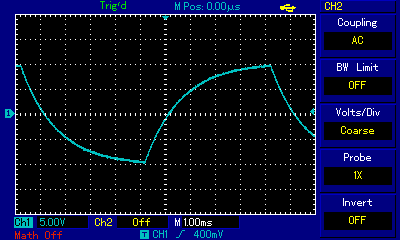
\includegraphics[width= 0.6\textwidth]{MAP001.png}
  \caption{Aufladekurve eines Kondensators über einen Widerstand}
  \label{abb:osz}
\end{figure}
\\
\\
\\
\begin{table}[h]
  \centering
  \caption{Messwerte zur Bestimmung der Zeitkonstante aus Aufladevorgang.}
  \label{tab:a}
   \begin{tabular}{c c}
     \toprule
    {$t $ \:/\: ms} & {$U_C $ \:/\: \si{\volt}}\\
    \midrule
    0.2\pm0.05 &  2.0 \pm0.05 \\
    0.4\pm0.05 &  4.2 \pm0.05 \\
    1.0\pm0.05 &  9.6 \pm0.05 \\
    1.2\pm0.05 &  11.0\pm0.05 \\
    1.4\pm0.05 &  12.2\pm0.05 \\
    1.6\pm0.05 &  13.2\pm0.05 \\
    2.0\pm0.05 &  14.8\pm0.05 \\
    2.6\pm0.05 &  16.6\pm0.05 \\
    3.0\pm0.05 &  17.4\pm0.05 \\
    3.4\pm0.05 &  18.0\pm0.05 \\
    3.8\pm0.05 &  18.4\pm0.05 \\
    4.0\pm0.05 &  18.6\pm0.05 \\
    4.4\pm0.05 &  19.0\pm0.05 \\
    4.8\pm0.05 &  19.2\pm0.05 \\
    \bottomrule
  \end{tabular}
\end{table}\\
Am Anfang wird die Formel \eqref{eqn:aufladung} in die folgegende
Form gebracht.
\begin{equation}
1-\frac{U_C}{U_0}=e^{-{\frac{1}{RC}\cdot t}}
\end{equation}
Zur Auswertung der ersten Messreihe wird der Logarithmus
von $1-\frac{U_C}{U_0}$ gegen die Zeit $t$ aufgetragen, wie in Abbildung \ref{abb:a} zu sehen.
\begin{equation}
  \ln \left(1-\frac{U_C}{U_0}\right)=-\frac{1}{RC}*t
\end{equation}
\begin{figure}[!h]
  \centering
  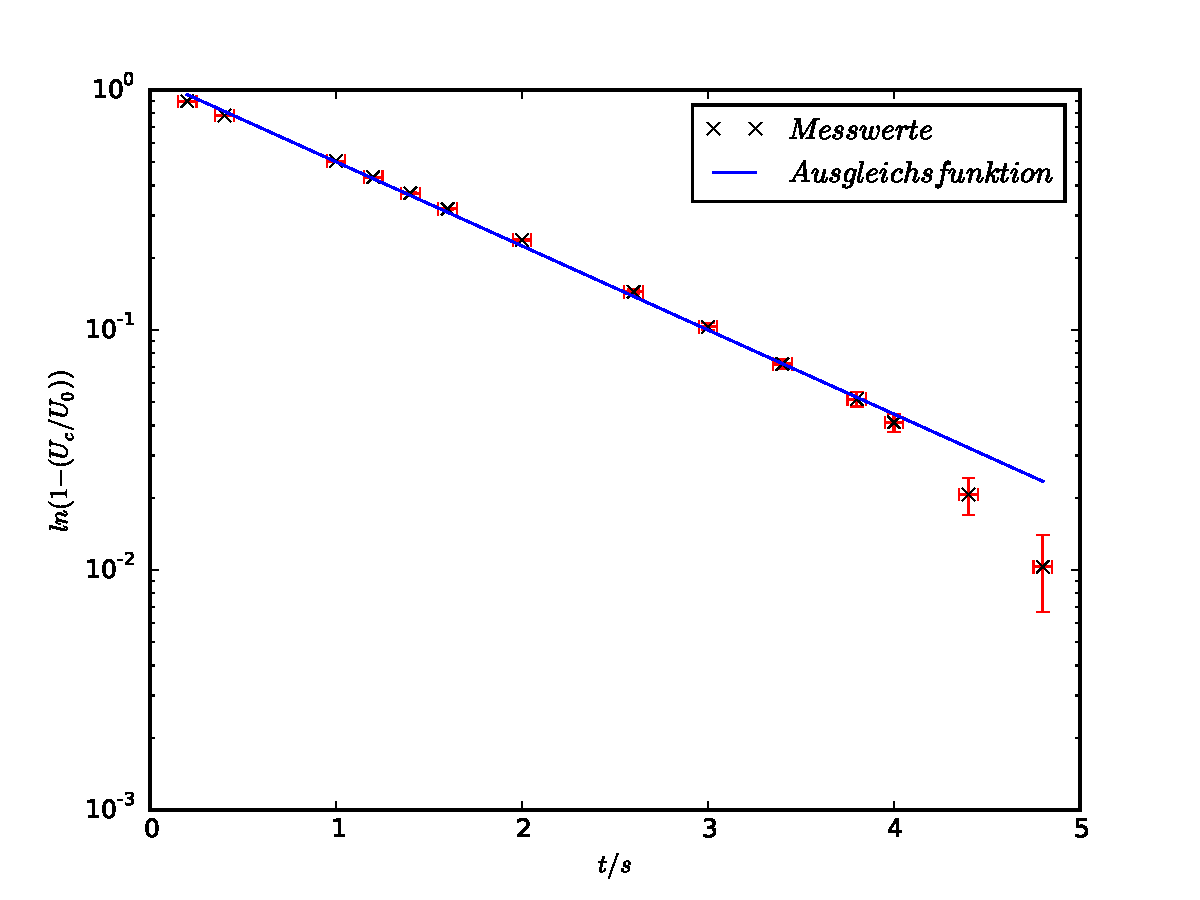
\includegraphics[width=0.7\textwidth]{a.pdf}
  \caption{Bestimmung von der $RC$-Konstant aus dem
  Aufladevorgang eines Kondensators}
\label{abb:a}
\end{figure}
\FloatBarrier
Zur Bestimmung der Zeitkonstante wird nun eine lineare Regression durchgeführt.
Das Ergebniss ist $1/RC$ als Steigung der Graden.
Der Kehrwert der Steigung ist nun die Zeitkonstante $RC$.\\
$RC$ ist hierbei $0.00111\pm0.05 s$
\\
\subsection{Bestimmung der Zeitkonstante mittels Frequenzabhängigkeit der Amplitude }
Erneut wird die Zeitkonstante bestimmt, nur diesmal unter
der Betrachtung von der Frequenzabhängigkeit von der Amplitude von $U_C$.
Die Amplitude wird halblogarithmisch gegen die Frequenz aufgetragen, und eine Ausgleichsrechnung
entsprechend der Gleichung \eqref{eqn:amplitude} wird durchgeführt,
diese Darstellung findet sich in Abbildung \ref{abb:b} wieder.
Die Messwerte befinden sich in Tabelle \ref{tab:b}.
Hier beträgt die Zeitkonstante $RC=0.000936 \pm 0.000000007s$
\begin{figure}[h]
  \centering
  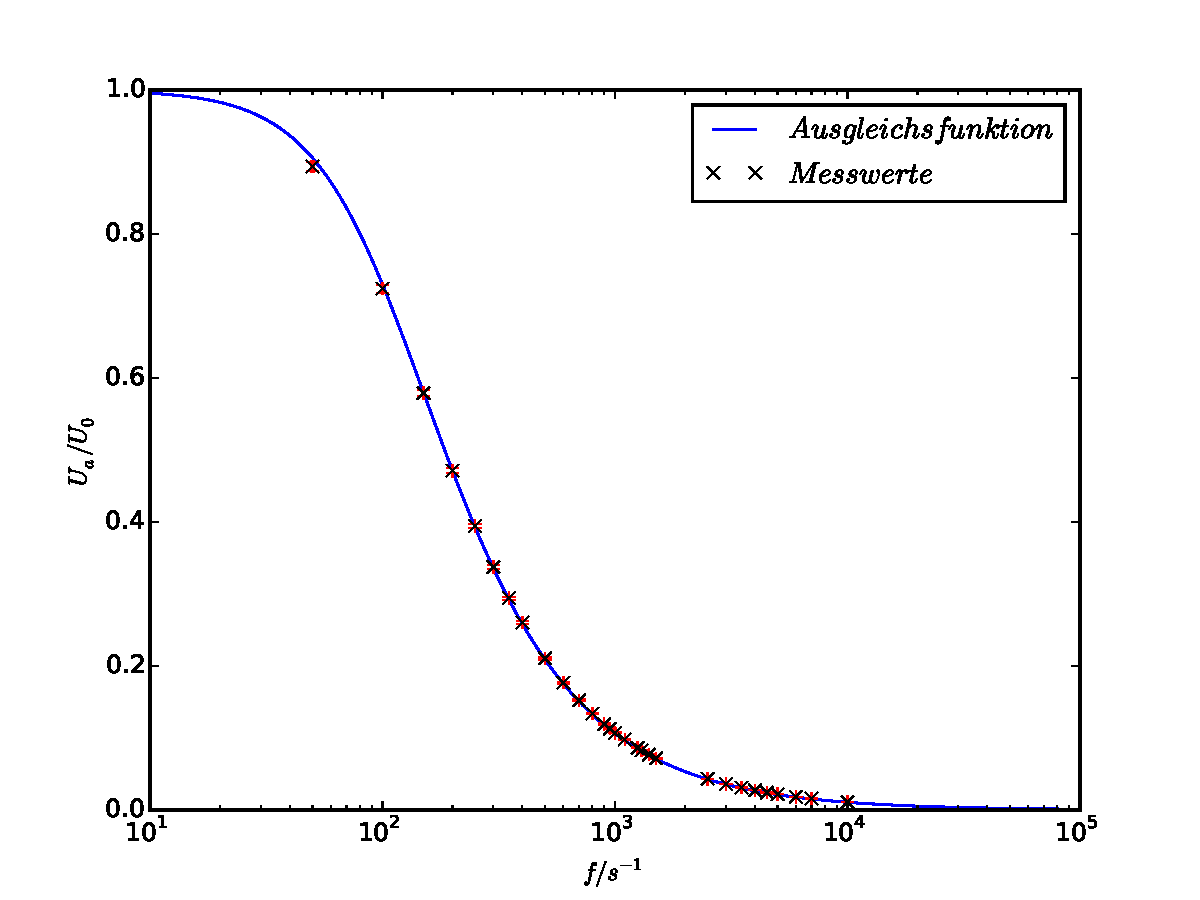
\includegraphics[width=1\textwidth]{b.pdf}
  \caption{$U_a/U_0$ in Abhängigkeit von der Frequenz $f$}
  \label{abb:b}
\end{figure}
\begin{table}[h]
  \centering
  \caption{Messwerte zur Bestimmung der Zeitkonstante aus Aufladevorgang.}
  \label{tab:b}
   \begin{tabular}{c c || c c}
     \toprule
    {$f $ \:/\: Hz} & {$A $ \:/\: \si{\volt}} & {$f $ \:/\: Hz} & {$A $ \:/\: \si{\volt}}\\
    \midrule
    50  \pm0.5 &   6.078\pm0.0005 &  1100\pm0.5 &   0.666\pm0.0005 \\
    100 \pm0.5 &   4.923\pm0.0005 &  1250\pm0.5 &   0.587\pm0.0005 \\
    150 \pm0.5 &   3.937\pm0.0005 &  1300\pm0.5 &   0.564\pm0.0005 \\
    200 \pm0.5 &   3.204\pm0.0005 &  1400\pm0.5 &   0.524\pm0.0005 \\
    250 \pm0.5 &   2.683\pm0.0005 &  1500\pm0.5 &   0.488\pm0.0005 \\
    300 \pm0.5 &   2.295\pm0.0005 &  2500\pm0.5 &   0.295\pm0.0005 \\
    350 \pm0.5 &   2.000\pm0.0005 &  3000\pm0.5 &   0.246\pm0.0005 \\
    400 \pm0.5 &   1.77 \pm0.0005 &  3500\pm0.5 &   0.211\pm0.0005 \\
    500 \pm0.5 &   1.432\pm0.0005 &  4000\pm0.5 &   0.186\pm0.0005 \\
    600 \pm0.5 &   1.202\pm0.0005 &  4500\pm0.5 &   0.166\pm0.0005 \\
    700 \pm0.5 &   1.036\pm0.0005 &  5000\pm0.5 &   0.149\pm0.0005 \\
    800 \pm0.5 &   0.91 \pm0.0005 &  6000\pm0.5 &   0.125\pm0.0005 \\
    900 \pm0.5 &   0.811\pm0.0005 &  7000\pm0.5 &   0.108\pm0.0005 \\
    950 \pm0.5 &   0.768\pm0.0005 &  10000\pm0.5 &   0.075\pm0.0005 \\
    1000\pm0.5 &   0.729\pm0.0005\\
  \bottomrule
  \end{tabular}
\end{table}
\\
\FloatBarrier
\subsection{Bestimmung der Zeitkonstante mittels Frequenzabhängigkeit der Phase}
Ein letztes Mal wird die Zeitkonstante bestimmt, diesmal mit Hilfe der Phasenverschiebung von Generator und Kondensartorspannung in Abhängigkeit von der Frequenz.
Die Werte aus Tabelle \ref{tab:c} werden gegeneinander Aufgetragen, wie in Abb.\ref{abb:c} .Die Phasenverschiebung $\phi$ wird für
die Tabelle nach Formel $\phi=\frac{a}{b}\cdot2\pi$ errechnet.
Das Ergebnis hierbei für Zeitkonstante RC ist $0.00087\pm0.0000002 s$
\begin{figure}[h]
  \centering
  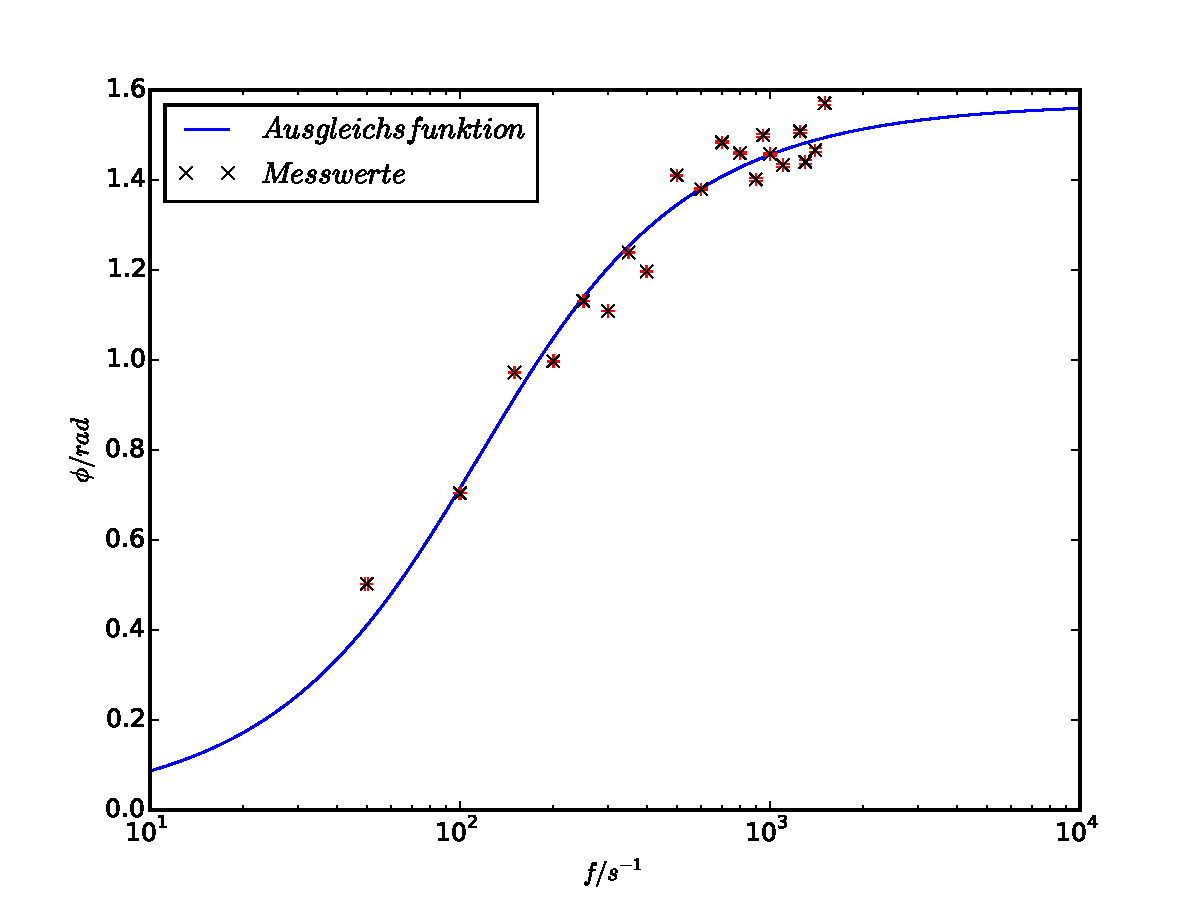
\includegraphics[width=1\textwidth]{c.pdf}
  \caption{Frequenz $f$ zur Phasenverschiebung $\phi$ aufgetragen}
  \label{abb:c}
\end{figure}
\begin{table}[h]
  \centering
  \caption{Messwerte zur Bestimmung der Zeitkonstante aus Aufladevorgang.}
  \label{tab:c}
   \begin{tabular}{c c c c}
     \toprule
    {$f $ \:/\: Hz} & {$ a $ \:/\: ms}  & {$ b $ \:/\: ms} & {$ \phi $ \:/\: $\pi$ } \\
    \midrule
    50.  \pm0.5 &  1.6  \pm0.0005 &      20. \pm0.0005   & 0.16\pm0.00005  \\
    100. \pm0.5 &  1.12 \pm0.0005 &    10.   \pm0.0005 & 0.22\pm0.0001 \\
    150. \pm0.5 &  1.04 \pm0.0005 &    6.72  \pm0.0005 & 0.31\pm0.0002 \\
    200. \pm0.5 &  0.8  \pm0.0005 &    5.04  \pm0.0005 & 0.32\pm0.0002 \\
    250. \pm0.5 &  0.72 \pm0.0005 &    4.0   \pm0.0005 & 0.35\pm0.0003 \\
    300. \pm0.5 &  0.6  \pm0.0005 &    3.4   \pm0.0005 & 0.39\pm0.0004 \\
    350. \pm0.5 &  0.56 \pm0.0005 &    2.84  \pm0.0005 & 0.38\pm0.0004 \\
    400. \pm0.5 &  0.48 \pm0.0005 &    2.52  \pm0.0005 & 0.45\pm0.0005 \\
    500. \pm0.5 &  0.44 \pm0.0005 &    1.96  \pm0.0005 & 0.44\pm0.0006 \\
    600. \pm0.5 &  0.36 \pm0.0005 &    1.64  \pm0.0005 & 0.47\pm0.0007 \\
    700. \pm0.5 &  0.34 \pm0.0005 &    1.44  \pm0.0005 & 0.46\pm0.0008 \\
    800. \pm0.5 &  0.288\pm0.0005 &    1.24  \pm0.0005 & 0.45\pm0.0009 \\
    900. \pm0.5 &  0.248\pm0.0005 &    1.112 \pm0.0005 & 0.48\pm0.001 \\
    950. \pm0.5 &  0.252\pm0.0005 &    1.056 \pm0.0005 & 0.46\pm0.001 \\
    1000.\pm0.5 &  0.232\pm0.0005 &    1.    \pm0.0005 & 0.46\pm0.001 \\
    1100.\pm0.5 &  0.208\pm0.0005 &    0.912 \pm0.0005 & 0.48\pm0.001 \\
    1250.\pm0.5 &  0.192\pm0.0005 &    0.8   \pm0.0005 & 0.46\pm0.001 \\
    1300.\pm0.5 &  0.176\pm0.0005 &    0.768 \pm0.0005 & 0.46\pm0.001 \\
    1400.\pm0.5 &  0.168\pm0.0005 &    0.72  \pm0.0005 & 0.47\pm0.001 \\
    1500.\pm0.5 &  0.168\pm0.0005 &    0.672 \pm0.0005 & 0.5\pm0.002 \\
    \bottomrule
\end{tabular}
\end{table}
\newpage
Nun werden die Werte mit identischer Frequenz
aus der Tabelle \ref{tab:b} und \ref{tab:c} in einem
Polarplott dargestellt wie in Abbildung \ref{abb:d} zu sehen.
\begin{figure}
\centering
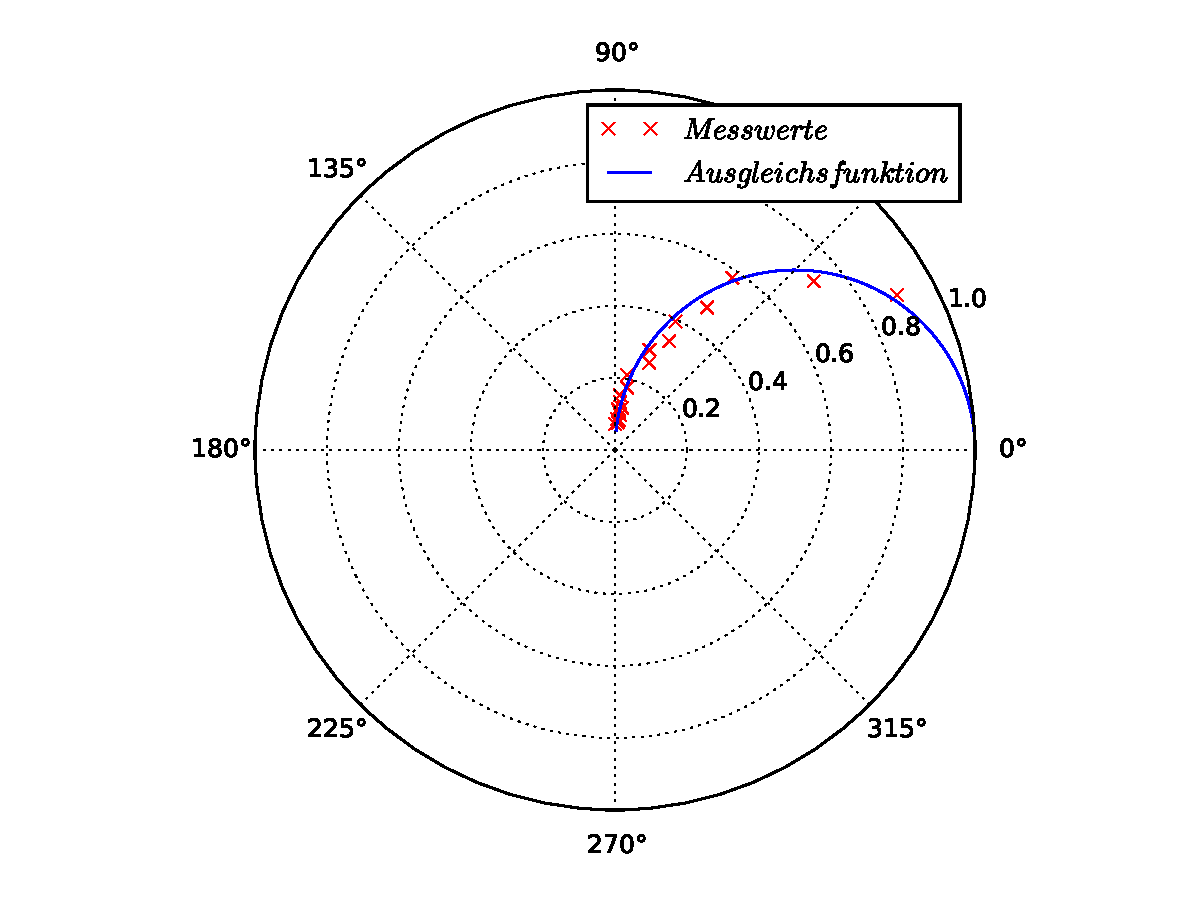
\includegraphics[width=0.8\textwidth]{d.pdf}
\caption{Amplitude $A_0$ in Abbhängigkeit von der Phasenverschiebung $\phi$ }
\label{abb:d}
\end{figure}
\FloatBarrier
\subsection{Eignung als Integrator}
Die folgenden Abbildungen zeigen die integrierten Kurven von Dreiecks-,Rechtsecks-und Sinusspannung.
Für eine Phase Sinusspannung, ergibt sich, wie in Abbildung \ref{abb:sinus} zu sehen, eine Cosinusspannung, dies entspricht auch der Stammfunktion:
\begin{align}
  f(x)&=a\cdot \sin{x}&F(x)&=-a\cdot \cos{x}.
\end{align}\\
Bei einer Phase der Rechtecksspannung ergibt sich als integrierte Spannung eine Grade mit konstanter Steigung,
zu erkennen anhand der Abbildung \ref{abb:rechteck} und der Stammfunktion:
\begin{align}
  f(x)=
  \begin{cases}
    a,& 0 \leq t \textless \pi\\
   -a,& -\pi \leq t \textless 0
  \end{cases}
  \ \ \ \ \ \ \ \ \
  F(x)=
  \begin{cases}
    a\cdot x,& 0 \leq t \textless \pi\\
   -a\cdot x,&  -\pi \leq t \textless 0.
  \end{cases}
\end{align}\\
Für eine Phase der Dreiecksspannung ergibt sich als integrierte Spannung eine Parabel, dies ist sowohl in Abbildung \ref{abb:dreieck} als auch anhand der Stammfunktion zu erkennen:
\begin{align}
  f(x)=
  \begin{cases}
    a\cdot x,& 0 \leq t \textless \pi\\
   -a\cdot x,&  -\pi \leq t \textless 0
  \end{cases}
  \ \ \ \ \ \ \ \ \
  F(x)=
  \begin{cases}
    \frac{a}{2}\cdot x^2,& 0 \leq t \textless \pi\\
   \frac{-a}{2}\cdot x^2,&  -\pi \leq t \textless 0.
  \end{cases}
\end{align}\\
\begin{figure}[h]
    \centering
    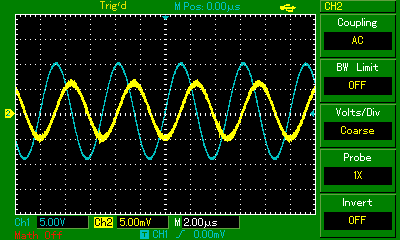
\includegraphics[width=0.6\textwidth]{MAP007.png}
    \caption{Bild der Sinusspannung und ihrer Integrierten Spannung.}
    \label{abb:sinus}
\end{figure}\\
\begin{figure}[h]
    \centering
    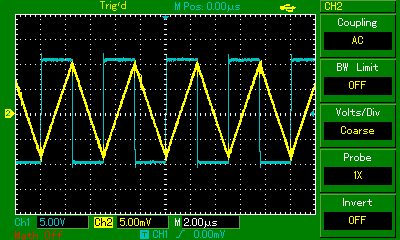
\includegraphics[width=0.6\textwidth]{MAP006.png}
    \caption{Bild der Rechteckspannung und ihrer Integrierten Spannung.}
    \label{abb:rechteck}
\end{figure}\\
\begin{figure}[h]
    \centering
    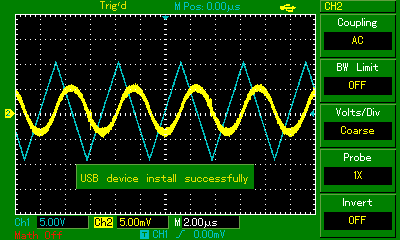
\includegraphics[width=0.6\textwidth]{MAP005.png}
    \caption{Bild der Dreicksspannung und ihrer Integrierten Spannung.}
    \label{abb:dreieck}
\end{figure}\\
